\chapter{绪论}

\section{引言}
子痫前期(preeclampsia, PE)又作先兆子痫,是孕妇妊娠期特有的一种多系统进展性疾病, 与妊娠期高血压(gestational hypertension)、子痫(eclampsia)、
慢性高血压并发子痫前期(chronic hypertension with superimposed preeclampsia)以及妊娠合并慢性高血压(chronic hypertension)统称妊娠期
高血压疾病(hypertension disorders of pregnancy, HDP)\cite{OAG9,HDASOM,2000s1}。
子痫前期临床表现的显著特点是原发性高血压与蛋白尿。
近年来,组织的对子痫前期的涵盖范围进行了进一步的拓展,在妊娠20周后出现新发(原发)高血压,在两次间隔$4h$或$4h$以上的血压测定中,收缩压≥$140mmHg$和(或)
舒张压≥$90mmHg$,且伴有下列任一项或多项\cite{OAG9,FIGO}:
\begin{itemize}
    \item 孕妇出现蛋白尿症状,尿蛋白≥$300mg/24h$,或尿蛋白/肌酸酐比值≥$30mg/mol$,或随机尿蛋白≥(+);
    \item 孕妇无尿蛋白但伴有以下任一器官或系统功能紊乱、受累受损:心、肺(肺水肿)、肝(血清转氨酶水平为正常值2倍以上)、肾(血肌酐水平大于$1.1mg/dl$
    或为正常值2倍以上)等重要器官,或血液系统(血小板<$100 \times 10^{9}/L$)等)、消化系统、神经系统的异常改变等;
    \item 胎盘-胎儿受到累及:胎盘胎儿生长受限、脐动脉多普勒分析检测异常、死胎等。 
\end{itemize}

妊娠期高血压疾病可引起严重的母胎并发症,是孕产妇和围产儿病死率升高的主要原因\cite{OAG9}。
据世界卫生组织统计,子痫前期在孕妇中发病率高达5\%-10\%,是除体内大出血外孕妇死亡的第二大危险因素\cite{LCT2006},每年可导致全球范围内约76 000名孕妇死亡,并进一步导致约500 000
名胎儿/婴儿的死亡\cite{DAM2015,LCT2006}(如\autoref{fig:dhd}所示)。为推广普及人们对危及母婴生命安全的子痫前期的认知,同时教育女性了解她们当前及长期的健康风险,
全球孕妇保健组织自2017年起将每年的5月22日确定为世界子痫日(world preeclampsia day)(如\autoref{fig:wpd}所示)。
\begin{figure}[htb]
    \centering
    \includegraphics[width=.7\linewidth]{ch1/dhd}
    \caption{\label{fig:dhd}因妊娠期高血压疾病死亡孕妇的国家分布比例}
\end{figure}
\begin{figure}[htb]
    \centering
    \includegraphics[width=.7\linewidth]{ch1/wpd}
    \caption{\label{fig:wpd}2021年世界子痫日主题:Preeclampsia: Beyond Pregnancy}
\end{figure}

就现阶段我国国情而言,由于人口基数大、人口出生率较高,导致每年妊娠孕妇数及新生儿数总量大。
同时,自全面开放二孩政策后,各地区高龄孕妇、二次妊娠孕妇比例明显提升。而临床研究已经证实,
高龄与二(三)次妊娠均属于可能导致子痫前期的风险因素,会增加孕妇子痫前期的患病可能。

因此,如何对子痫前期快速有效的医学诊断与干预成为新的难题,实现子痫前期的预测和及早诊断,
是对孕妇子痫前期的治疗及孕妇、围生儿的健康安全的保障,具有重大的临床应用价值。
\section{子痫前期的病理及危害}
\subsection{病因及发病机制}
截止目前,医学界对子痫前期的病因与发病机制尚未完全明确,相关研究还在继续进行之中。但得到公认的一点是,子痫前期病发具有异质性,多因素、多机制及多通路均对子痫前期的发病有所影响,不能仅以“一元论”的观点对待。
目前最为普遍接受的一种观点认为,子痫前期的发病与妊娠早期胎盘功能紊乱密切相关,其作用机制可以概括为两个阶段,如\autoref{fig:ppp}所示。
在第一阶段,孕妇子宫螺旋动脉重构受损、出现重铸障碍,导致胎盘缺血、缺氧,释放多种胎盘因子,该阶段无明显临床现象;在第二阶段,各种胎盘因子进入母体血液循环,促进系统性炎症反应的激活及血管内皮损伤引起子痫前期-
子痫多样化的临床表现。有关病因和发病机制的主要学说有以下几种:
\begin{figure}[htbp]
    \centering
    \includegraphics[width=.7\linewidth]{ch1/ppp}
    \caption{\label{fig:ppp}一种子痫前期可能的发病机制}
\end{figure}

(一)子宫螺施小动脉重铸不足:

正常妊娠时,细胞滋养层细胞分化为绒毛滋养细胞和绒毛外滋养  第一阶段t1细胞(extravillous trophoblast,EVT),EVT包括间质第三阶1般氧化应激及胎盘浅猪床-「无临床征象
.绒毛外滋养细胞(interstitial extravillous trophoblast.
费症反应
1出现临床征乘
EVT)和血管内绒毛外滋养层细胞(endovascular ex-
travillous trophoblast,enEVT),iEVT负责浸润子宫1母体全身炎症反应
内膜基质直至子宫肌层的内1/3处,enEVT则进入
子宫螺旋小动脉管腔并逐渐替代血管壁平滑肌细
全身小动脉痉率1胞、内皮细胞,使动脉由高阻力低容量血管转变为
子梅前期-子痛
低阻力高容量血管以提高胎盘的血流量、确保母胎 图8-4 子痢前期发病机制“两阶段学说”示意图之间物质交换正常进行和胎儿发育。但子痫前期绒毛外滋养细胞泻
和子宫螺旋动脉重铸极其不足,仅蜕膜层血管重铸,子宫螺旋动脉1已完成等级加速,活跃天数1阻力增大,胎盘灌注减少,从而引发子痫前期的一系列症状。但造成子宫螺旋小动脉重铸 足的机制尚待研究。


(二)炎症免疫过度激活

子痫前期患者无论是母胎界面局部还是全身均存在炎症保中激活现象。现有证据显示,母胎界面局部处于主导地位的天然免疫系统在子痫前期发病中起重要作用,Toll样受体家族、蜕膜自然杀伤细胞(dNK)、巨噬细胞等的数量、表型和功能异常均可影响子宫螺旋小动脉重铸,造成胎盘浅着床。特异性免疫研究集中在T细胞,正常妊娠时母体Th1/Th2免疫状态向Th2漂移,但子痫前期患者蜕膜局部T淋巴细胞向Thl型漂移。近年发现,CD4"CD25"调节性T细胞(regulatory T cell,Treg细胞)参与Thl/Th2免疫状态的调控。当Treg细胞显著减少时,促进Thl占优势,使母体对胚胎免疫耐受降低,引发子痫前期。

认为胎儿胎盘是具有半抗原性移植体,妊高征实质上是胎儿胎盘对母体诱导出的较强的免疫应答反应。精子内有组织相容性抗原(HLA)存在,如胎儿胎盘遗传得到HLA者,HLA处于免疫惰性状态,故能支持母亲免疫系统接受胎儿胎盘异体移植物,
反之,则可引起母体抗原抗体反应。临床上妊高征患者HLA抗体的检出率明显高于正常孕妇,妊高征患者蜕膜及胎盘血管动脉粥样硬化病变与移植器官时的血管病变相似;妊高征患者体液免疫与细胞免疫功能异常等,都支持免疫学说。

(三)血管内皮细胞受损

血管内皮细胞损伤是子痫前期的基本病理变化之一,它使扩血管物质如一氧化氮(NO)、前列环素,合成减少,而缩血管物质如内皮素(ET)、血栓索A,等合成增加,从而促进血管痉挛。此外血管内皮损伤还可激活血小板及凝血因子,加重子痫前期的高凝状态。引起子痛前期血管内皮损伤的因素很多,如炎性介质:肿瘤坏死因子、白细胞介素-6、极低密度脂蛋白等,还有氧化应激反应。

妊娠期多数凝血因子增加,凝血功能增加,纤溶活性抑制,血液处于高凝状态。妊高征患者上述变化更显著,抗凝血酶(ATⅢ)减少,血容量减少,血液浓缩,加之血管痉挛,内皮损伤,胶原暴露,易出现血栓。缺血缺氧之胎盘变性坏死,释放促凝物质进入母体血循环,激发血管内凝血。妊高征患者血中纤维蛋白降解产物(FDP)增高,血小板减少,凝血功能检查异常,甚至有出血倾向,肾小球纤维蛋白沉积,胎盘梗死等均支持DIC学说。但妊高征与DIC的因果关系尚未肯定。


(四)遗传因素

子痫前期具有家族倾向性,提示遗传因素与该病发生有关,但遗传方式尚不明确。由于子痫前期的异质性,尤其是遗传和环境因素的交互作用产生了复杂的表型。在子痫前期遗传易感性研究中,尽管目前已定位了十几个子痛前期染色体易感区域,但在该区域内进一步寻找易感基因仍面临很大的挑战。

(五)其他学说

近几年来,学者们还相继提出一些新的可能引起子痫前期的学术观点,如前列腺素合成失调与孕妇营养不足等。前列腺素合成失调观点认为当孕妇血液中具有血管收缩作用的血栓素(TXA2)增高而具有扩张血管作用的前列环素(PGI2)相对不足时,
则易导致血管痉挛、血压升高从而最终引发子痫前期。同时一些临床研究也发现,多种营养因素如低白蛋白血症、钙、镁、锌、硒等缺乏与子痫前期发生发展可能有关。但此类学说与假设仍需进一步临床研究与理论研究来证实。

\subsection{子痫前期引起的生理变化及危害}
妊高征基本的病理生理变化是全身小动脉痉挛和水钠潴留。

(一)全身小动脉痉挛 可能由于升压系统和降压系统平衡失调,血管壁对某些升压物质(如血管紧张素Ⅱ)的反应性增强,从而使全身小动脉,特别是直径200um以下的小动脉发生痉挛,导致各器官供血不足,外周阻力增高,产生高血压等一系列症状体征。

子宫血管痉挛,胎盘供血不足,绒毛退行性变、出血、坏死、梗塞等,导致胎盘提高老化,功能不全。病变进行缓慢时,可致胎儿宫内生长发育迟缓(IUGR),病变急剧时,可致胎死宫内,严重时胎盘后小血管破裂,导致胎盘早剥。

脑部血管痉挛,脑组织缺氧、水肿、严重时出血,出现头昏、头痛、恶心、呕吐,重者抽搐、昏迷,脑疝形成而致死亡。

心脏血管痉挛,心肌缺血、间质水肿、点状出血及坏死,加之血液粘稠度增加,外周阻力增加,心脏负担加重,可导致左心衰竭,继而发生肺水肿。

肾脏血管痉挛,肾血流量减少,组织缺氧,血管壁通透性增加,血浆从肾小球漏出,出现蛋白尿及管型。肾小球毛细血管痉挛,肾小球内皮细胞肿胀,发生血管内凝血,纤维蛋白沉着,肾小球滤过率减少,出现尿少,严重者出现肾功衰竭。

肝脏由于缺血,肝细胞线粒体内所含的谷丙转氨酶释放,可致血清谷丙转氨酶升高,出现黄疸表明病情严重。肝脏主要病变为门静脉周围有局限性出血,继而纤维素性血栓形成,严重者肝实质缺血坏死、肝包膜下出血。

眼底小动脉痉挛、缺血、水肿,严重时渗出、出血,甚至视网膜剥离,出现眼花、视物模糊,甚至失明。

(二)水钠潴留 可能由于肾小球滤过率减少,肾小管对钠的重吸收增加,钠离子潴留细胞外而引起水肿。肾上腺皮质激素、抗利尿激素分泌增加,也可能是水潴留的另一个原因。由于水钠潴留,组织水肿,体重异常增加。

【病理生理变化及对母儿影响】
-基本病理生理变化是全身小血管痉挛和血管内皮损伤。全身各脏器各系统灌注减少,对母儿造成危害,甚至导致母儿死亡。由于该病表现为多脏器和系统损害,故有学者提出子痫前期-子痫综合征(preeclampsia-eclampsia syndrome)的概念。
1,脑 脑血管痉挛,通透性增加,导致脑水肿、充血、局部缺血、血栓形成及出血等。CT检查脑皮质呈现低密度区,并有相应的局部缺血和点状出血,提示脑梗死,并与昏迷及视力下降、失明相关。大范围脑水肿主要表现为感觉迟钝和思维混乱,个别患者可出现昏迷,甚至脑疝。子病前期脑血管阻1力和脑灌注压均增加,高灌注压可致明显头痛而子痫的发生与脑血管自身调节功能丧失相关。
2肾脏肾小球扩张,内皮细胞肿胀,纤维素沉积于内皮细胞。血浆蛋白自肾小球漏出形成蛋 m
尚未明确。

\section{子痫前期的研究现状}
现代医学对子痫前期的认知经历了漫长的探索\cite{BJOG2016}。
\subsection{参数}
\subsection{设备}
\subsection{分析技术}
\subsection{发展史}
\subsection{风险因子}
庄彩霞等人\cite{Zhuang2019}对中国境内的98 000余例分娩孕妇进行了分析,得出了中国人群子痫前期的主要独立风险因子包括:慢性高血压疾病、既往子痫前期病史、$BMI≥28kg/m^2$、肾脏疾病、多胎妊娠、心脏病、$BMI 24~28kg/m^2$等。
\subsection{血压}
\subsection{生化指标}
生化指标(biomarker)
123

\begin{figure}[htbp]
    \centering
    \includegraphics[width=.3\linewidth]{ch1/aocheng_kit}
    \caption{\label{fig:aocheng_kit}胎盘生长因子检测试剂盒}
\end{figure}
123

\subsubsection{1}

\subsection{人工智能技术}
近年来,由于现代化设备的普遍使用致使医学检查过程各项数据激增,同时计算机领域人工智能技术的不断创新发展,相关研究者也开始尝试在子痫前期的识别、判断乃至预测等研究内容上引入人工智能技术。
2016年,Rutvij Mehtad等\cite{Mehta2016}将大数据挖掘技术(Major Data Mining)在预测子痫前期、产科风险因素及产科其他疾病等健康领域的主要研究进行了归纳总结。他们将诸多学者的研究涉及的
数据挖掘与分析总结为两大类应用研究方向,即关联规则挖掘方向与分类、聚类分析方向。关联规则挖掘力求发现多项数据之间的隐藏的逻辑与关系;分类分析是对通过现有数据建立模型预测新数据所属类别,
聚类分析则是按照一定规则将所有数据分组,使每组内的数据尽可能相似并有别于其他组数据\cite{Han2006}。在两大类应用的基础上,学者们使用不同的数据对子痫前期进行了分析研究。

2021年,Rong Guo等人\cite{Guo2021}构建了C4.5决策树(decision tree, DT)、自适应增强(adaptive boost, AdaBoost)及多层感知机(multilayer perceptron,MLP)三种分类器,利用集成学习投票决策,
从众多胎盘$mRNA$表达基因样本中筛选出了识别子痫前期的最佳生化指标,成功地将原始48个指标降维至13个,同时将分类识别准确性从开始的$79\%$提高至$82.2\%$。

2005年,Louise C. Kenny等人从代谢组学

Surama Biswas等人
\begin{figure}[htbp]
    \centering
    \includegraphics[width=.6\linewidth]{ch1/ai}
    \caption{\label{fig:ai}部分对子痫前期的机器学习研究}
\end{figure}


\subsection{设备技术}
(一)血管回声跟踪技术(echo tracking,ET)
张秀丽等人\cite{Zhang2014}利用超声技术对孕妇颈动脉弹性进行了检测,研究发现子痫前期孕妇颈总动脉内膜厚度无显著性差异,但反应血管弹性的指标会有一定程度的改变,具体表现为僵硬系数、压力应变弹性系数及脉搏波传播速度升高和顺应性系数降低,
对包括子痫前期在内的孕高症的防治具有一定程度的指导意义。


\subsection{存在的不足与分析}
综合上述分析,对子痫前期的早期识别与检测可从按以下思路开展深入探索与研究。



\section{脉搏波在子痫前期领域研究现状}
用脉搏波检测子痫的优势:

DM Carty等人对脉搏波增强指数(augmentation index,AIx)进行了研究,
Kathleen Tomsin等人\cite{Tomsin2012}对脉搏波传输时间参数(pulse transit time, PTT)进行了研究,结果显示除肝静脉和胸主动脉外,子痫前期的早期(n=12)及晚期患者(n=14)的PTT较正常孕妇(n=16)数值更低。
Feng Jiang等人基于光电容积脉搏波提出了一种新型形态学特征分层面积比(hierarchical area ratio,HAR)参数。
2018年,Ying Feng等人提出

2014年,Ira Bernstein等\cite{Ira2014}人通过34名孕妇在孕早期(PRE)、12-14孕周(V2)及30-32孕周(V3)的手腕脉搏波PWV数据及心脏射血时间进行了测量与分析,结果发现子痫前期患者较正常孕妇,其PWV数值在V3期数值往往更大,
(pre- eclampsia: 0.121?0.113 vs. Controls: 0.139?0.132 secs; p¼.04)。


\section{研究目标与内容}

\subsection{研究目标}
综合应用各种方法,提取研发新型光电容积脉搏波形态学特征参数,构建一般通用的光电容积脉搏波的描述特征集合。在此基础上,通过特征筛选、压缩等算法提取出对子痫前期有一定甄别能力的特征集,
使用机器学习算法构建出子痫前期筛选识别模型,并对最终模型的性能表现进行验证评估。
\subsection{研究内容}
全文研究内容可分为数据源获取、信号预处理、特征参数提取与分析、子痫前期甄别模型训练构建及模型评估具体包括5个部分,如所示。每部分具体研究内容包括:
\begin{enumerate}
    \item 数据源获取。介绍本研究所采用的数据来源(临床现场采集),包括采集设备、采集流程及规范。  
    \item 信号预处理。对从硬件设备获取的PPG信号分析其信号成分特点,完成滤波去噪、去基线漂移、特征点检测及标准化等准备工作。
    \item 特征参数提取与分析。从脉搏波形态学等方面构建特征参数。
    \item 子痫前期甄别模型训练构建及评估。通过机器学习中的等方法构建子痫前期甄别模型,并验证模型准确性。
    \item 模型评估。
\end{enumerate}

\textbf{各章节的具体内容安排如下:}

第一章是绪论。介绍子痫前期的定义及危害,梳理了目前临床已应用的检测方法及指标,分析各项方法的缺陷与不足。最后确定提出了本文的研究目标与内容。

第二章是光电容积脉搏波概述。阐述了

第三章是光电容积脉搏波的特征点检测算法。

第四章是光电容积脉搏波的特征集构建。

第五章是基于光电容积脉搏波特征的子痫前期检测识别模型。通过等几种方法优化特征参数集并构建了子痫前期的甄别模型,通过等方面评估了各项模型的整体性能表现。

第六章是低耦合高拓展的软件综合分析系统的设计与实现。阐述了本研究包括数据源导入管理、预处理算法管理、特征拓展管理、标准数据管理、模型训练生成管理等方面在内的整体分析系统的软件设计思路,
介绍了为提高本研究各部分内的内聚性、降低各研究内容之间的耦合性、提高系统整体可拓展性及实用性、提高系统真正落地临床的可能性所做出的各项规划及实现。

第七章是总结与展望。对本论文的全部研究工作进行系统性总结,阐述本论文的创新工作点,并对下一阶段的研究工作内容进行了规划与展望。

\chapter{光电容积脉搏波概述}
\section{引言}
由于本研究开展所使用的脉搏波数据均为通过光电容积描述标记的方法无创所得,因此在本章最后进一步阐述了微循环容积脉搏波血流模型及光电容积脉搏波采集原理。
\section{脉搏波产生原理}
\section{生理参数与非生理参数建立的心血管模型}
按照信号与系统的观点,若干相互作用、相互联系的事物按一定规律组成具有特定功能的整体均可称为系统,而信号则是反映信息的各种物理量,是系统直接进行加工、变换以实现通信的对象。而在脉搏波的工程研究领域,
人体的动脉管系亦可视为一个力学系统,心脏搏动作为该系统输入,而人体各处采集获得的脉搏波即为该系统输出(响应)。可由该系统的输入输出关系分析推断其结构特性参数,进一步研究脉搏波其他特性。\cite{PPGYY}

为尽可能精确描述心血管系统、探求心血管系统的生理特性,多年来学者们提出并建立了各种不同的数学模型进行拟合。而这些心血管模型大体上可依据建立时是否使用多个变量去拟合还原血液在血管中的可能涉及的血压、
血流弹性、阻力等生理变量分为生理参数模型与非生理参数模型两大类\cite{PPGYY}。生理参数模型关注心血管系统中的所有细节,模型中的各个参数变量均有较好的解释,也能与实际生理病理现象有较好的对应;而非生理参数则是
使用黑箱方法,不追求任何细节,仅通过输入输出信息来研究推导心血管系统模型,具有建立模型过程简单同时不破坏系统任何原有结构等优势。本节后续将分别从两大类模型中各选取一种经典模型进行介绍。
\subsection{双弹性腔模型}
双弹性腔模型最早由等人于1963年提出q
对于第一个弹性腔室,血液输入输出关系满足:
\begin{equation}
    \label{equ:QS1}
    q_{in}-q=\frac{\mathrm{d} V_{1}}{\mathrm{d} t}
\end{equation}
对于第一个弹性腔室,血液输入输出关系满足:
\begin{equation}
    \label{equ:QS2}
    q-q_{out}=\frac{\mathrm{d} V_{2}}{\mathrm{d} t}
\end{equation}
设腔室容积$V$与压力$p$之间为线性关系,则有:
\begin{equation}
    \label{equ:QSV1}
    \frac{\mathrm{d} V_{1}}{\mathrm{d} t}
    =\frac{\mathrm{d} V_{1}}{\mathrm{d} p_{1}}\frac{\mathrm{d} p_{1}}{\mathrm{d} t}
    =c_{1}\frac{\mathrm{d} p_{1}}{\mathrm{d} t}
\end{equation}
\begin{equation}
    \label{equ:QSV2}
    \frac{\mathrm{d} V_{2}}{\mathrm{d} t}
    =\frac{\mathrm{d} V_{2}}{\mathrm{d} p_{2}}\frac{\mathrm{d} p_{2}}{\mathrm{d} t}
    =c_{2}\frac{\mathrm{d} p_{2}}{\mathrm{d} t}
\end{equation}
不失一般性,设腔体1、2之间的血液流淌在长度为$l$,截面积为$A$的刚性管道之中。依据动量守恒,则有:
\begin{equation}
    \label{equ:QM}
    \frac{\mathrm{d}}{\mathrm{d} t}\left ( \rho Al\frac{q}{A} \right )=p_{1}A-p_{2}A
\end{equation}
其中,$\rho$为血液密度,$q$为容积流量,$q/A$为血流速度。
\autoref{equ:QM}可进一步简化为
\begin{equation}
    \left \{
    \begin{aligned}
        L\frac{\mathrm{d} q}{\mathrm{d} t} &= p_{1}-p_{2} \\
        L &=\rho \frac{l}{A} \text{(血流惯性)}
    \end{aligned}
    \right.
\end{equation}
设弹性腔压力$p_{2}$和流入血管床的血流$q_{out}$之间为线性关系,即
\begin{equation}
    \label{equ:pq}
    q_{out}=\frac{p_{2}}{R}
\end{equation}
则系统的状态方程可写成
\begin{equation}
    \left \{
    \begin{aligned}
        \frac{\mathrm{d} q}{\mathrm{d} t} &= \frac{1}{L}(p_{1}-p_{2}) \\
        \frac{\mathrm{d} p_{1}}{\mathrm{d} t} &= \frac{1}{C_{1}}(q_{in}-q) \\
        \frac{\mathrm{d} p_{2}}{\mathrm{d} t} &= \frac{1}{C_{2}}(q-\frac{p_{2}}{R}) \\
    \end{aligned}
    \right.
\end{equation}
进一步化简,消除$q$、$p_{1}$可得到:
\begin{equation}
    \label{euq:diff}
    \frac{\mathrm{d^3} p_{2}}{\mathrm{d} t^3}+\frac{1}{RC_{2}}\frac{\mathrm{d}^2p_{2} }{\mathrm{d} t^2}+
    (\frac{1}{LC_{1}}+\frac{1}{LC_{2}})\frac{\mathrm{d} p_{2}}{\mathrm{d} t}+\frac{1}{LRC_{1}C_{2}}p_{2}
    =\frac{1}{LC_{1}C_{2}}q_{in}
\end{equation}
求解该线性三阶微分方程的特征方程,可得
\begin{equation}
    \label{euq:character}
    S^3+\frac{1}{RC_{2}}S^2+(\frac{1}{LC_{1}}+\frac{1}{LC_{2}})S+\frac{1}{LRC_{1}C_{2}}=0
\end{equation}
该特征方程的解由三个分量组成,即直流分量、非震荡衰减分量和震荡衰减分量三部分,可对脉搏波的主波、潮波和重博波等主要特征点进行较好的描绘。

\subsection{自回归滑动平均模型}
由于脉搏波信号具有较强的随机性,且其时变特性符合平稳随机信号的定义,因此,我们可以采用平稳随机信号的线性模型对脉搏波进行建模分析\cite{TJXHCL,PPGYY}。在此基础上,脉搏波信号$X(n)$可以看作是某一线性系统在
白噪声$W(n)$的激励下而得到的响应。只要确定了白噪声的相关参数,我们便可以将对平稳随机信号PPG的研究转换成对随机信号的线性系统的研究,典型的随机信号参数模型如所示。

根据系统传递函数形式的不同,可以将平稳随机信号的线性参数模型分为滑动平均(moving average,MA)模型,自回归(autoregressive,AR)模型及自回归滑动平均模型(autoregressive moving average,ARMA)模型等三种。其中,
ARMA模型是AR模型与MA模型的组合,表示脉搏波信号$X(n)$是由自身若干过去值$X(n-k)$与激励时的白噪声$W(n)$及若干白噪声过去值$W(n-k)$线性组合产生的,即:
\begin{equation}
    \label{equ:ARMA}
    X(n)=-\sum_{k=1}^{p}a_{k}X(n-k)+\sum_{k=0}^{q}b_{k}W(n-k)
\end{equation}
对\autoref{equ:ARMA}进行$z$变换,则可得到ARMA模型的传递函数为:
\begin{equation}
    \label{equ:ARMAH}
    H(Z)=\frac{X(Z)}{W(Z)}=\frac{\sum_{k=0}^{q}b_{k}Z^{-k}}{1+\sum_{k=1}^{p}a_{k}Z^{-k}}=\frac{B(Z)}{A(Z)}
\end{equation}
可知,ARMA模型既有零点,也有极点,是零极点模型,一般记作$ARMA_{(p,q)}$,其中$p$与$q$分别是AR模型与MA模型的阶次。
对\autoref{equ:ARMA}进行傅里叶变换,可进一步得到ARMA模型的功率谱估计为\cite{TJXHCL}:
\begin{equation}
    \label{equ:ARMAP}
    \hat{P}_{ARMA}(e^{j\omega} )=
    \delta _{\omega}^2\left |  \frac{\sum_{k=0}^{p}\hat{b}_{k}e^{-j\omega}}{\sum_{k=0}^{q}\hat{a}_{k}e^{-j\omega}}\right |^2
    =\delta _{\omega}^2\left |  \frac{\hat{B(e^{j\omega} )}}{\hat{A}(e^{j\omega} )}\right |^2
\end{equation}

与上小节中的双弹性腔三阶模型类似,实际证明当采用ARMA的三阶模型$ARMA_{(3,2)}$来拟合实际脉搏波波形时,模型输出与实测波形拟合度高、误差小\cite{PPGYY}。在此情形下,脉搏波波形可由源自\autoref{equ:ARMA}的
\begin{equation}
    \label{equ:ARMA32}
    \begin{aligned}
        X(n)=&-a_{1}X(n-1)-a_{2}X(n-2)-a_{3}X(n-3)\\
        &+b_{0}W(n)+b_{1}X(n-1)+b_{2}W(n-2)
    \end{aligned}
\end{equation}
来表征。则模型的传递函数为
\begin{equation}
    \label{equ:ARMAH32}
    \begin{aligned}
        H(Z)&=\frac{X(Z)}{W(Z)}=\frac{b_{0}+b_{1}Z^{-1}+b_{2}Z^{-2}}{1+a_{1}Z^{-1}+a_{2}Z^{-2}+a_{3}Z^{-3}}\\
        &=g_{0}+g_{1}Z^{-1}+g_{2}Z^{-2}+...+g_{N-1}Z^{N-1}
    \end{aligned}
\end{equation}
其中,$g_{i}$为脉搏波实际采样数值,$N$为采样点数。
此时,求解模型则转换成求解\autoref{equ:ARMA32}中相应的$a_{i}$、$b_{i}$,使模型拟合曲线与原曲线均方差和最小,即满足:
\begin{equation}
    \label{equ:MeanSum}
    \Delta_{min}=\sum_{i=1}^{N}\left |  (g_i-g'_i)^2\right |
\end{equation}
其中$g'_i$为模型拟合数值。
\section{微循环容积脉搏波血流模型}
与上一小节类似,微循环容积脉搏波血流模型亦可用生理参数模型与非生理参数模型来描述。由于非生理参数模型本身就是黑箱模型,故上小节中ARMA模型在此完全适用,本小节不再赘述。
但微循环的生理参数模型则需进行一定的修正和补充。

根据输入输出关系及该过程中动量守恒,可到微循环弹性腔血流模型的数学表达式为
\begin{equation}
    \label{equ:wxh1}
    \left \{
    \begin{aligned}
        \frac{\mathrm{d} Q}{\mathrm{d} t} &=\frac{P_{in}-P}{L}\\
        \frac{\mathrm{d} P}{\mathrm{d} t} &=\frac{Q-Q_{out}}{C}\\
        Q_{out} &=\frac{P}{R}
    \end{aligned}
    \right.
\end{equation}
消去$P$、$Q$,同样可得一线性三阶微分方程:
\begin{equation}
    \label{equ:wxh2}
    \frac{\mathrm{d^2} Q_{out}}{\mathrm{d} t^2}+\frac{1}{RC}\frac{\mathrm{d} Q_{out}}{\mathrm{d} t}+\frac{1}{LC}Q_{out}=\frac{1}{RLC}P_{in}
\end{equation}
易得其传递函数为
\begin{equation}
    \label{equ:hs}
    \begin{aligned}
    G(s) &=\frac{Q_{out}(s)}{P_{in}(s)}=\frac{\frac{1}{RLC}}{S^2+\frac{1}{RC}S+\frac{1}{LC}} \\
    &=\frac{1}{RLC}\frac{1}{2\sqrt{(\frac{1}{2RC})^2-\frac{1}{LC}}}(\frac{1}{S-S_{1}}-\frac{1}{S-S_{2}})
    \end{aligned}
\end{equation}
其中,
\begin{equation}
    \label{equ:ss}
    \left \{
    \begin{aligned}
        S_{1} &= -\frac{1}{2RC}+\sqrt{(\frac{1}{2RC})^2-\frac{1}{LC}}\\
        S_{2} &= -\frac{1}{2RC}-\sqrt{(\frac{1}{2RC})^2-\frac{1}{LC}}\\
    \end{aligned}
    \right.
\end{equation}
\section{光电容积脉搏波采集原理}
光电容积脉搏波描记法(Photoplethysmography,PPG)最早于1938年由Hertzman等人提出,利用光电转换方法检测组织中血液容积变化的一种技术。由于采集测量过程无创、无痛、迅速、便捷等特性,PPG技术已经在临床
普及,成为各种监护设备必备的监测参数之一\cite{ldl,lhc}。

PPG检测可依据光的接收方式分为透射式与反射式两种\cite{THOCBPM},透射式PPG采集原理是使用一定波长光源照射在人体组织表面,由于皮肤、血液、肌肉等各组织的吸收,一部分光发生漫反射,
一部分投过组织被传感器接收,其中光源与传感器对称分布;反射式工作原理与透射式基本相同,区别在于传感器被放置光源同侧接收漫反射回来的光\cite{THOCBPM,mmt},如\autoref{fig:led}所示。
透射式PPG检测一般多用于人体耳垂、指端等部位,反射式PPG一般多用于手腕、
胸部等其他表层血管发达区域\cite{THOCBPM}。一般认为,透射式检测更方便指示心率的时间关系,而反射式则对于血管容积变化的检测更有优势\cite{mmt}。
\begin{figure}[htb]
    \centering
    \includegraphics[width=.7\linewidth]{ch2/led}
    \caption{\label{fig:led}PPG检测的两种方式}
\end{figure}

当心脏收缩时外周血容量最多,光吸收量也最大,故检测到的光强度最小;而在心脏舒张时则恰恰相反,外周血容最小,光的吸收量最小,检测到的光强度最大\cite{lhc,cwl}。
由于人体指端区域毛细血管组织发达等优点,因此在光电容积脉搏波的临床中成为了检测位置的首选。\autoref{fig:ppgab}展示了人体指端各组织对光的吸收情况。
\begin{figure}[htb]
    \centering
    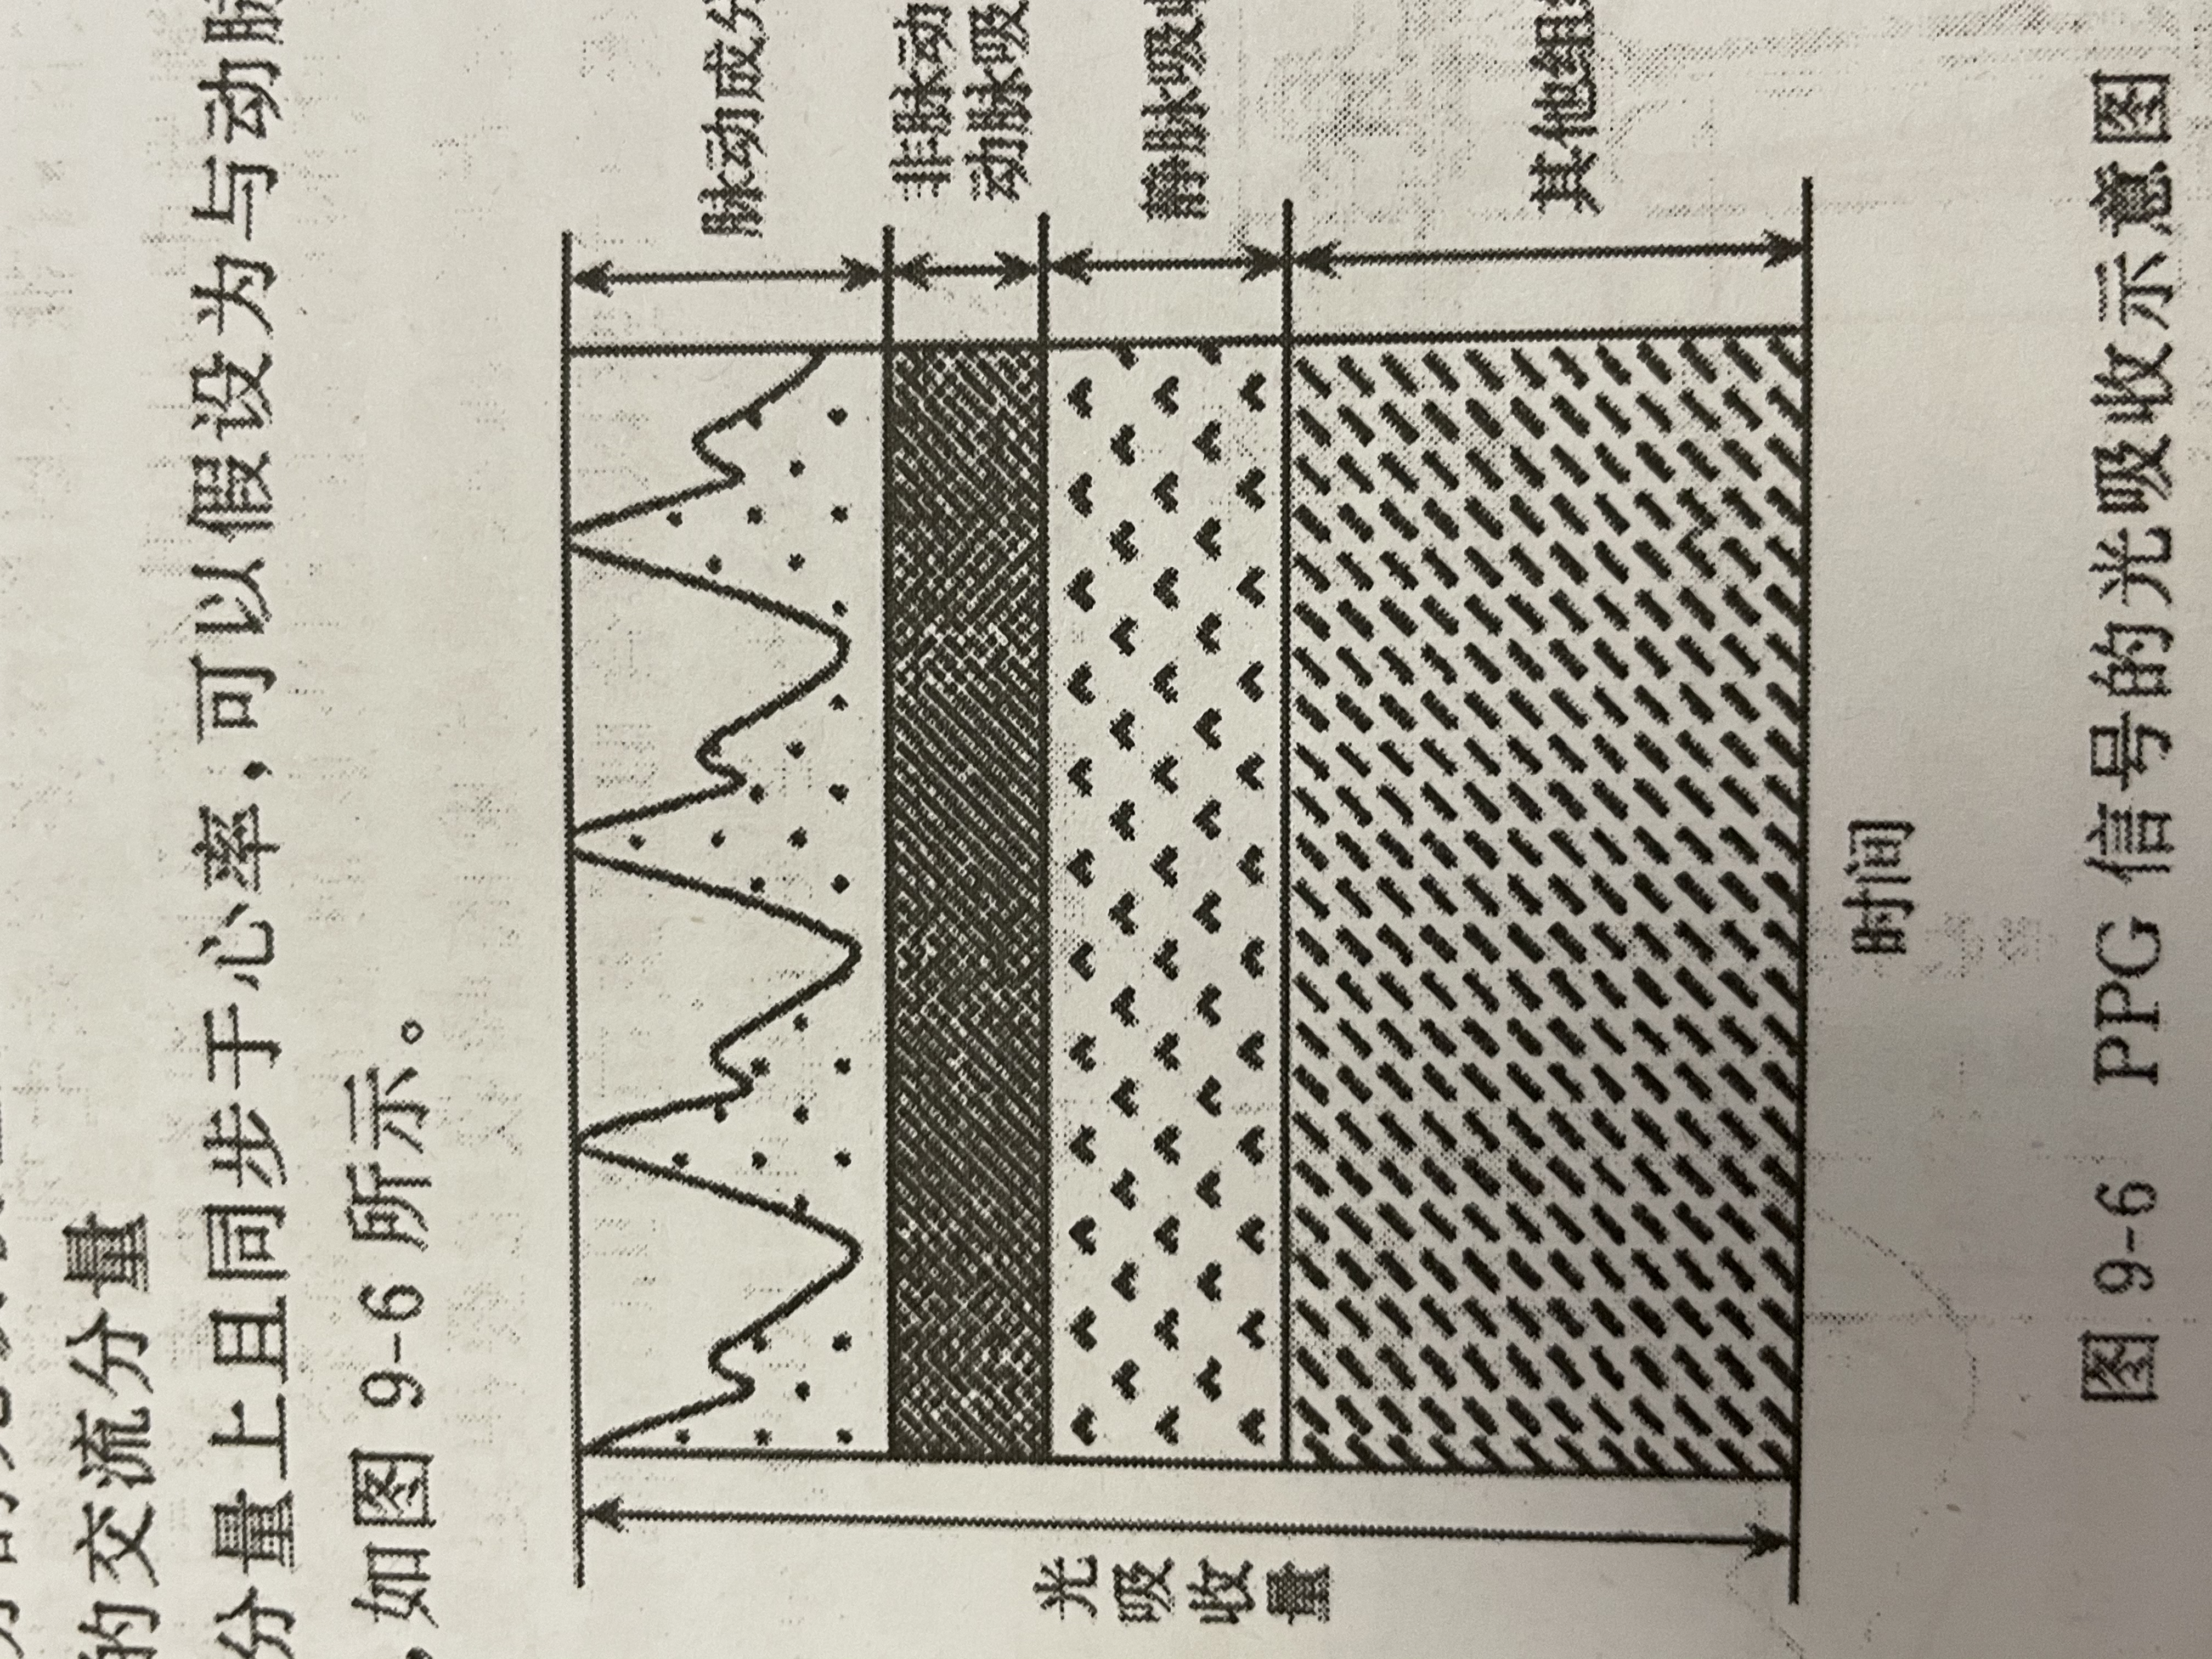
\includegraphics[width=.7\linewidth]{ch2/ppgab}
    \caption{\label{fig:ppgab}PPG信号的光吸收示意图}
\end{figure}

具体而言,物理光学中,将光通过某种透明介质后被吸收的比例定义为光的吸收度$A$,即:
\begin{equation}
    \label{equ:LBL}
    A=\lg\frac{I_{0}}{I_{T}}
\end{equation}

其中,$I_{0}$与$I_{T}$分别是入射光强度与透射光强度。而朗伯-比尔定律(Lambert-Beer's law)指出,光的吸收度与入射光的强度无关,在光程上每等厚层介质吸收相同比例值的光,即:
\begin{equation}
    \label{equ:LBL2}
    A=C \cdot \varepsilon \cdot V
\end{equation}

其中,$V$是透明介质的体积,$C$是透明介质的浓度,$\varepsilon$则是吸收系数,一般与透明介质的性质、入射光波长及温度等因素相关。

在透射式的光电检测中考虑到人体指端各组织对入射光的均有吸收,若忽略由于散射、反射等因素造成的衰减,以波长为$\lambda$的单色光垂直照射指端,则最终指端透射光强度为\cite{4122392}:
\begin{equation}
    \label{equ:AF1}
    I=I_{0}e^{-C_{t}\varepsilon _{t}V_{t}}e^{-C_{v}\varepsilon _{v}V_{v}} e^{-C_{a}\varepsilon _{a}V_{a}} 
\end{equation}

其中,下标$t$、$v$、$a$分别代表皮肤肌肉组织、静脉血液、动脉血液等成分。学者们已经证实皮肤肌肉组织、静脉血液等组织对光的吸收是恒定不变的\cite{1980Spectrophotometric,4122392}。
因此,可对\autoref{equ:AF1}进行精简,以表示通过动脉血液的透光强度\cite{PPGYY}:
\begin{equation}
    \label{equ:AF2}
    I=I_{0}e^{-C_{a}\varepsilon _{a}V_{a}} 
\end{equation}

当动脉血液的容积因心脏搏动而发生极小的变化$\Delta V_{a}$时,透光强度也将随之变动,将其记为$\Delta I$,则\autoref{equ:AF2}可改写为:
\begin{equation}
    \label{equ:AF3}
    I+\Delta I=I_{0}e^{-C_{a}\varepsilon _{a}(V_{a}+\Delta V_{a})} 
\end{equation}

将\autoref{equ:AF2}与\autoref{equ:AF3}相除,可得:
\begin{equation}
    \label{equ:AF4}
    \frac{I+\Delta I}{I}=\frac{I_{0}e^{-C_{a}\varepsilon _{a}(V_{a}+\Delta V_{a})}}{I_{0}e^{-C_{a}\varepsilon _{a}V_{a}}}=e^{-C_{a}\varepsilon _{a}\Delta V_{a}} 
\end{equation}

进一步,对\autoref{equ:AF4}两边同时取对数,并根据数学近似关系,若$x\rightarrow 0$,则$\ln(1+x)\approx x$,可得:
\begin{equation}
    \label{equ:AF5}
    \frac{\Delta I}{I}=-C_{a}\varepsilon _{a}\Delta V_{a}
\end{equation}

将\autoref{equ:AF2}代入\autoref{equ:AF5},稍作整理可得:
\begin{equation}
    \label{equ:AF6}
    \frac{\Delta V_{a}}{V_{a}}=\frac{1}{\ln(I/I_{0})}\frac{\Delta I}{I}
\end{equation}

即与个体相关性强的动脉血总的光吸收系数$\varepsilon _{a}$、动脉血浓度$C_{a}$等变量最终均与指端血液容积变化率无关,而后者与该容积透射的光强变化率$\Delta I/I$成正比例关系,从而排除了个体差异等因素的影响
\cite{1980Spectrophotometric,4122392,PPGYY}。PPG信号检测正是依此原理,通过光电转换硬件电路检测光信号并从光强变化率中获取指端血液容积变化率的信息。
\section{典型光电容积脉搏波波形特征}
\section{脉搏波时域特征研究现状}
\section{小结}

\chapter{光电容积脉搏波数据源}
\section{引言}
\section{数据来源}
\section{人口统计学特征}
\section{采集设备}
\section{采集流程}
\section{脉搏波数据导出}
\section{小结}


\chapter{脉搏波特征点检测及特征参数集的构建}
\section{引言}
\section{信号预处理}
\section{脉搏波波形检测及纠错}
\section{时域特征参数设计与特征集构建}
\subsection{角度、幅值、长度等}
\section{小结}

\chapter{基于数据特征集的模型构建及评估}
\section{引言}

\section{数据来源}
\section{构建方法分析}
\section{模型构建}
\section{评估方式与标准}
\section{具体模型表现对比}
\section{小结}

\chapter{低耦合、高拓展的软件综合分析系统的设计与实现}
\section{背景分析}
* 子痫前期检测的特定场景:孕妇、高龄、周期长、时间

* 实验室已有前期硬件研究基础,家俊研究基础

\section{需求分析:模块化、低耦合、高拓展}
* 多场景

* 特征计算拓展

* 数据管理

* 模型识别判断

\section{整体设计框图展示}

\section{各模块具体设计}
* 硬件采集支持

* 对数据源的拓展——多种数据格式均可兼容

* 对数据预处理的拓展——波形定位算法可拓展、纠错算法可拓展

* 对数据类型的拓展——目前只涉及脉搏波,但可方便拓展ECG等信号

* 对特征集构建拓展——方便随时研发新的特征参数进入特征集

\section{实现展示与测试}
界面
输入输出
\section{小结}

\chapter{总结与展望}
\section{研究工作总结}
\section{主要创新点}
* 提出了多种新型脉搏波特征参数,从时域形态特征方面构建了一般通用的脉搏波特征集

* 从特征集中筛选出对子痫前期具有识别能力的有效特征集合,并基于有效特征集合通过机器学习方法构建了子痫前期综合预测模型

* 设计并实现了一种低耦合、高拓展的方便类似研究工作开展的软件综合分析系统

\section{下一阶段工作展望}


% \begin{algorithm}

% \end{algorithm}